\documentclass{article}
\usepackage{enumitem}
\usepackage{amsmath,amssymb,graphicx}
\usepackage[totalheight=9in, totalwidth=6in]{geometry} % config dimensions
\usepackage{cite}
%\usepackage{Sweave}
\usepackage{tikz}
\usepackage[english]{babel}
\usepackage{hyperref}
\usetikzlibrary{positioning,shapes.geometric,decorations.text}
\begin{document}
%\Sconcordance{concordance:Project-Proposal.tex:Project-Proposal.Rnw:%
1 2 1 1 0 64 1}


\newcommand{\E}{\mathbb{E}}
\newcommand{\indp}{\ensuremath{\perp\hspace{-5pt}\perp}}
\newcommand{\M}{\mathcal{M}}
\newcommand{\given}{\; \mid \;}



\title{\textbf{The Effect of Dieting on Sleep}}
\author{Alex Luedtke, Lucia Petito, and Steven Pollack}
\date{}
\maketitle

\section{Specify the Question}

Recently researchers have tried to relate successful dieting to sleeping habits.  A relationship between obesity and sleep cycles has been established: both oversleeping \cite{sgain} and sleep deprivation \cite{sloss} are associated with an increased Body Mass Index (BMI). 

Nonetheless, little work has been done to consider the converse relationship. Specifically, we are interested in parsing the causal effect of attempting to lose weight on a person's sleep habits (average hours of sleep/night). While the health benefits associated with losing weight are well documented, it is not currently known if dieting has any effect on an individual's sleep habits.

There are reasonable explanations for all possible outcomes of this analysis.  An increased interest in one's diet could indicate an increased interest in one's overall health.  Because doctors advise their patients to consistently get enough sleep each night to maintain a healthy lifestyle, it would be reasonable to see more hours of sleep in people who are dieting.  On the other hand, dieting has profound psychological and hormonal effects \cite{hormone}, which could cause a disruption to normal sleep patterns and result in less sleep on average.

For the purposes of this analysis, our population of interest is adults ages 25-79 who are not pregnant, have never been diagnosed by a doctor with a sleep disorder, and live in the United States.  We used the National Health and Nutrition Examination Survey (NHANES) data from 2009-2010 \cite{data} from the ``Demographic Variables and Sample Weights," ``Weight History 16 Years and Older," and ``Sleep Disorders" questionnaires \cite{questionnaire}.

NHANES is a multi-stage survey of the U.S. population that the Center for Disease Control and Prevention (CDC) conducts every 2 years.  Figure \ref{fig:survey.design}  shows the survey design as visualized on the NHANES website.  Counties are sampled first, then ``segments'' (which can be as small as street blocks to as big as neighborhoods: determined by population density), then households, and finally individuals.  Because such a multistage suvey design does not yield a simple random sample from the population, NHANES supplies survey weights for each individual which are supposed to approximately represent the proportion of the population of which an individual is representative. Specifically, incorporating these survey weights is supposed to help remove bias from resulting estimates so that the conclusions drawn from the study are generalizable to the more general population of interest.

The study aims to consider a wide range of topics such as cardiovascular disease, obesity, physical fitness and physical functioning, reproductive history and sexual behavior, etc.  Each individual participates in an interview and a physical examination.  The sample is chosen to represent the U.S. population of all ages.  To produce reliable statistics, NHANES over-samples persons 60 and older, adolescents, African Americans, and Hispanics among others \cite{survey}.  


\begin{table}
\centering
\begin{tabular}{| p{3cm} | p{8cm} |}
\hline
When the interview was conducted & 1 for November 1, 2009 - April 30, 2010, 2 for May 1, 2009 - October 31, 2010\\
\hline
Subject Gender & 1 for Male, 2 for Female\\
\hline
Age in Months & 300-959, or 25-79 years\\
\hline
Race/Ethnicity & 1 for Mexican American, 2 for Other Hispanic, 3 for Non-Hispanic White, 4 for Non-Hispanic Black, 5 for Other Race\\
\hline
Education Level & 1: less than 9th grade, 2: 9-11th grade (including 12th grade with no diploma), 3: high school grad/GED or equivalent, 4: some college or AA degree, 5: college graduate or above\\
\hline
Marital Status & 1: married, 2: widowed, 3: divorced, 4: separated, 5: never married, 6: living with partner\\
\hline
Annual Household Income & 14 levels, \$0-\$24,999 by \$5,000, \$25,000-\$74,999 by \$10,000,  \$75,000 - \$99,999, \$100,000 and over, \$20,000, \$20,000\\
\hline
Body Mass Index & continuous values from ~15-50 [Note: this is a combination of subject weight and subject height, computed according to the formula used by the CDC \cite{bmi}\\
\hline
\end{tabular}
\caption{Baseline Covariates}
\label{tab:Covariates}
\end{table}


To protect the privacy of the participants, the CDC strips the data of any information that would allow an analyst to find an individual.  This process primarily removes geographic identifiers. In particular, all information about the first three stages of their multistage sampling procedure is removed.  Unfortunately, this removal of information means that we cannot fully replicate their sampling methodology. In particular, we were uncertain about our ability to perform a consistent bootstrap procedure.
Table \ref{tab:Covariates}  lists all of the baseline covariates we deemed relevant to our question that were available in NHANES.  In an ideal experiment we would want to include several additional covariates that were unfortunately not available in the questionnaires, including but not limited to a mental illness diagnosis, a prescription for medicine that affects sleep cycles as a side effect, and an average of how many hours per day the individual watches television/uses other electronic devices with screens.  Although we believe these factors heavily influence sleep patterns, we were not able to include them in our analysis.

This data set contains many individuals with missing data.  The percentage missing in each covariate is in Table \ref{tab:percent.missing}. Of particular concern is the fact that our intervention of interest, namely whether or not an individual tried to lose weight in the last year, is missing in more than 10\% of people sampled.  We implemented a complete-case analysis instead of implementing an imputation procedure for this study. Specifically, we deleted all people who responded ``refused" or ``don't know" or are missing data for Annual Household Income, Marital Status, Education Level, and Interview Time Period.  We deleted all people who were younger than 25 and older than 79, all pregnant women, and all people who had ever been diagnosed by a doctor with a sleep disorder (or who responded that they ``don't know").  We acknowledge that handling missigness in this way may lead to systematic bias unless the data are missing completely at random.

\begin{table}
\centering
\begin{tabular}{|l|l|}
\hline
Variable & \% Missing \\
\hline
Exam Date & 1.87 \\
Gender & 0 \\
Age & 0 \\
Race/Eth & 0 \\
Education & 0 \\
Relationship? & 0 \\
Income & 0 \\
BMI & 3.93 \\
\hline
Tried to lose weight? & 12.03 \\
\hline
Avg Hours of Sleep & 0.19 \\
\hline
\end{tabular}
\caption{Marginal percent missing for each variable considered after restricting to our population of interest of non-pregnant individuals between 25 and 79 years old without sleep disorders.}
\label{tab:percent.missing}
\end{table}

We also coarsened the categories for several of the variables in Table \ref{tab:Covariates} .  We were interested in the ``Marital Status'' variable because it described whether or not the individual had a stable relationship in their life, so we collapsed it into ``married or living with partner'' vs ``else.''  Because a significant number of people replied ``above \$20,000'' and ``below \$20,000'' to the annual household income question, we decided to define all individuals as such, including those for which we had more detailed information.  We also collapsed the bottom two categories for ``Education Level'' into one category: ``less than 12th grade.''

\section{Specify the Causal Model}

Our observational data structure is $O=(W,A,Y) \sim P_0$. Our endogenous variables are $W$, $A$, and $Y$, where $W$ is as listed in Table \ref{tab:Covariates}  with the modified categories specified at the end of the previous sectoin.

The intervention $A$ is the individual's response to the survey question: ``During the past 12 months, have you tried to lose weight?". The response $Y$ is the individual's response to the question: ``How much sleep do you usually get at night on weekdays or workdays?''  

Our exogenous variables are $U = (U_W, U_A, U_Y) \sim P_U$. We make no assumption on the joint distribution of $U$. Furthermore, we make no exclusion restrictions between our variables and no assumptions on the functional forms of $W$, $A$, or $Y$.

Because the data for $W$, $A$, and $Y$ was gathered simultaneously, temporal assumptions are needed to specify a causal model. Specifically, we assume that all variables in $W$ occur temporally before the variables in $A$ and $Y$, and that $A$ occurs before $Y$. Towards a temporal ordering between $W$ and $A$, we see that a subject's gender, age, race, and BMI one year ago must appear before their decision to diet in the last twelve months. Hence, a temporal ordering between these covariates and $A$ is plausible. Also, the date of the interview must occur before the answer to the question in $A$. Thus, we have temporal ordering here as well. Nonetheless, we do not necessarily have temporal ordering for education level, marital status, and annual household income. Thus we cannot be certain that all of $W$ can be placed before $A$. Nonetheless, switching the time ordering so that some $V\subset W$ occurs after $A$ is even more questionable, as education level, marital status, and annual household income are all somewhat unlikely to have changed within the last year. Thus we must go forward making the temporal assumption between $W$ and $A$. Note that all of the same observations hold for potential problems in the temporality between $W$ and $Y$.

Now, temporal assumptions between $A$ and $Y$ are somewhat justifiable due to the wording of the question in $A$. Specifically, the question asks whether the individual has tried to lose weight in the last year. The variable $Y$, on the other hand, asks about average sleep habits, which we believe indicates a response to a more recent phenomenon than the last year. Nonetheless, violations of this temporality may occur if the individual started to try to lose weight recently or if the individual considers long-term (more than a month) sleep habits when answering the question in $Y$. Though our temporality between $A$ and $Y$ is by no means perfect, we believe this temporal ordering is far more likely than the reverse, namely $Y\rightarrow A$. 

We now proceed, taking our temporal assumptions as given and the following SCM and the DAG as seen in Figure \ref{fig:DAG}:

\begin{align*}
W &= f_{W}(U_{W}) \\
A &= f_{A}(W,U_{A}) \\
Y &= f_{Y}(W,A,U_{Y}) \\
\end{align*}


\section{Specify the Causal Parameter of Interest}

Since the intervention is a point treatment, our counterfactual is $Y_{a}$: the average sleep an individual would get, if they, possibly contrary to fact, had (or had not) attempted to lose weight.

We are interested in measuring the average treatment effect (ATE) of attempting weight loss on average sleep:

$$\Psi(P_{U,X}) = \E_{P_{U,X}}[Y_1] - \E_{P_{U,X}}[Y_0]$$

\section{Assess Identifiability and Positivity}
\label{sec:assumptions}

Since $\Psi$ is the ATE, satisfying the backdoor criterion will identify G-computation with $\Psi$:
   $$Y_{a} \indp A \mid W$$

For identfiability, we need $U_{A} \indp U_{Y}$. [To see the modified DAG, see Figure \ref{fig:DAG1}] .  That is, we need there to be no unmeasured common causes between attempting to lose weight and average number of hours of sleep per weekday night. We also need either 
    \begin{itemize}
      \item $U_{A} \indp U_{W}$: No unmeasured common causes between an individual's attempt to lose weight and their baseline covariates. This assumption is somewhat plausible given the number of baseline covariates measured, but may not hold.
      \item $U_{W} \indp U_{Y}$: No unmeasured common causes between average hours of sleep per weekday night and baseline covariates. This assumption seems less plausible. For instance, an individual's stress level one year ago likely has a causal effect on their current relationship status and household income. This variable also likely has a causal relationship with current stress, which in turn may modify sleep habits.
    \end{itemize}

We must also address the issue of positivity.  We do not believe that trying to lose weight or not trying to lose weight occurs with probability $0$ given any set of covariates $W$ in our observed data distribution.  Thus we believe our theoretical positivity requirements are met.  However, practical positivity violations are very prevalent given that $W$ is high dimensional.  If we only consider those variables in $W$ that are categorical (Gender, Race/Ethnicity, Education Level, Marital Status), Table \ref{tab:prac.pos}  shows that we only have two strata where no people tried to lose weight. When the categorical variable for interview period is also considered, thirteen strata have practical positivity violations.

To get a better sense of the presence of near-practical positivity violations in our sample, see our discussion of the weight distribution in Figure \ref{fig:weight.dist} .

\begin{table}[ht]
\centering
\begin{tabular}{| l | l | l | l |}
\hline
 Gender & Race & Education & Marital Status \\
\hline
Male & Other & Less than HS & Unmarried/not living with partner \\
Female & Other & HS & Married/living with partner \\
\hline
\end{tabular}
\caption{Practical positivity violations that results when the categorical variables Gender, Race/Ethnicity, Education Level, Marital Status are considered.}
\label{tab:prac.pos}
\end{table}

\section{Commit to a Statistical Model and Target Parameter of the Observed Data Distribution}

We still have no assumptions on the functional forms of $f_W, f_A$, and $f_Y$, so we choose the non-parametric model $\mathcal{M}$ of distributions compatible with our SCM.  

We are still interested in the ATE, so our target parameter of the observed data distribution (assuming that we have a simple random sample) is

$$\psi_0 = \sum_{w}\Big[\E_0(Y|A=1,W=w)-E_0(Y|A=0,W=w)\Big]P_0(W=w)$$

\section{Estimate the Chosen Parameter of the Observed Data Distribution}
\label{sec:estimates}

We proceed with estimation although we cannot fully accept $U_A \indp U_W$ or $U_W \indp U_Y$ as presented in Section \ref{sec:assumptions}. If the assumptions hold, then we know that our estimates are directly estimating a causal parameter. Otherwise, we consider the estimates valuable pieces of information, albeit with known shortcomings. We will estimate the ATE using the following estimators: 

\begin{itemize}
  \item Simple Substitution:
    \[
      \psi_0 \approx \frac{1}{n}\sum_{i=1}^{n}\Big(\bar{Q}_{n}^{0}(1,W_i) - \bar{Q}_{n}^{0}(0,W_i)\Big)
    \]
Where $\bar{Q}_{n}^{0}(a,W_i)$ is an estimate of $\E_0(Y|A=a,W)$.
  \item IPTW:
  \[
    \psi_{0} \approx \frac{1}{n}\sum_{i=1}^{n} \left(\frac{I(A_i=1)}{\hat{g}_n(A_i \mid W_i)} - \frac{I(A_i=0)}{\hat{g}_n(A_i \mid W_i)} \right)Y_i
  \]
Where $\hat{g}_n(a_i \mid W_i)$ is an estimate of $P_0(A=a_i|W_i)$.
  \item TMLE:
  \[
    \psi_{0} \approx \frac{1}{n}\sum_{i=1}^{n}\left( \bar{Q}_{n}^{1}(1,W_i) - \bar{Q}_{n}^{1}(0,W_i)\right)
  \]
Where $\bar{Q}_{n}^{1}(a,W_i)$ is a targed estimate of $\E_0(Y|A=a,W)$ \cite{tmle}.
\end{itemize}

To incorporate survey weights, we take all of the means above to be weighted means, multiplying each term in the sums by the survey weight corresponding to that individual and then replacing the leading term $1/n$ with $1/S$, where $S$ represents the sum of all survey weights.

We obtain our estimates, $\hat{g}_{n}$ and $\bar{Q}_{n}^0$, using the candidate library in SuperLearner shown in Table \ref{tab:sl.lib} \cite{superlearner}. To calculate $\hat{g}_{n}$, we remove $A$ from all of the custom GLM's in the second column of Table \ref{tab:sl.lib}. Note that our SuperLearner includes both basic prediction algorithms such as SL.mean and more complex prediction algorithms such as SL.ridge and SL.glmnet. We have already described most of the algorithms listed here in a previous assignment, so will not do so here. We chose our custom GLM's to round out our library since fitting GLM's is a computationally inexpensive and easily implemented exploratory procedure. While the $Y \sim A \times Gender \times AgeMonths \times HHInc$ GLM would likely overfit the data if fit on the full data set, SuperLearner should overcome this problem data adaptively using cross-validation.

\begin{table}[tbp]
\centering
\begin{tabular}{l | l}
Default Algorithms & Custom GLM's \\
\hline
SL.mean & $Y \sim A$ \\
SL.earth & $Y \sim A \times Gender \times RaceEth + MarStat \times HHInc$ \\
SL.rpartPrune & $+ AgeMonths$:$Gender + EduLevel + AgeMonths $ \\
SL.ridge & $Y \sim A \times Gender \times MarStat$ \\
SL.glmnet &  $Y \sim A \times Gender \times AgeMonths \times HHInc$ \\
\end{tabular}
\caption{SuperLearner library. Note that the library includes both simple functions such as SL.mean and the custom $Y\sim A$ and higher level functions such as SL.earth (similar to SL.polymars) and SL.rpartPrune.}
\label{tab:sl.lib}
\end{table}

Figure \ref{fig:weight.dist}  shows that the weight distribution is fairly controlled, without too many large outliers. Because we truncated the x-axis for Figure \ref{fig:weight.dist} to make visualizing the distribution more feasible, we also show the summary of the distribution in Table \ref{tab:weight.summary}. Specifically, we see that the discrepancy between mean and median indicates a right-skewed distribution and that the largest weight is only 35.335.

\begin{table}[tbp]
\centering
\begin{tabular}{cccccc}
  \hline
 Min. & 25\% & Median & Mean & 75\% & Max. \\ 
  \hline
 1.037   & 1.281   & 1.587   & 1.952   &  2.198   &  35.335   \\ 
   \hline
\end{tabular}
\caption{Summary of distribution of weights. A truncated via of this distribution can be seen in Figure \ref{fig:weight.dist}.}
\label{tab:weight.summary}
\end{table}

We performed an unweighted bootstrap procedure to compute confidence intervals for the three estimators. In a follow-up analysis we included the survey weights to obtain point estimates for the simple substitution, IPTW, and TMLE estimators. We did not attempt to perform a weighted bootstrap procedure for these estimates as we were not sure how to use (and modify) the weights in a way that accurately recreated the survey design. Thus, rather than present uninterpretable confidence intervals, we will simply present the point estimates derived from the weight-conscientious analysis and compare them to the estimates that did not incorporate the survey weights.

A presentation of the empirical bootstrap sampling distributions can be found in Figure \ref{fig:weight.dist}. Note that the bootstrap distributions look fairly normal, which is supported in the Q-Q plots in Figure \ref{fig:qqplot}.

The point estimates and summaries can be found in Table \ref{tab:ests}. The point estimates   can be interpreted as the difference between the expected average number of additional hours of sleep that each individual will have if the entire population tries to lose weight and if the entire population does not try to lose weight. Visualizations of the confidence intervals appear in Figure \ref{fig:cis}. Note that the TMLE estimate is fairly unaffected by the consideration of survey weights, while the simple substitution and IPTW estimators increase and decrease, respectively.

\begin{table}[hbt]
\centering
\begin{tabular}{| l| l | l | l | l |}
  \hline
 & Weights? & Estimate & 95\% Normal CI & 95\% Quantile CI \\ 
  \hline
Simple Sub & No & 0.00983 & (-0.05444, 0.07411) & (-0.04403, 0.07961) \\ 
& Yes & 0.01733 & & \\
\hline
  IPTW & No & 0.38282 & (0.13473, 0.63091) & (0.40209, 0.89568) \\ 
& Yes & 0.16785 & & \\
\hline
  TMLE & No & 0.08175 & (-0.01418, 0.17769) & (-0.01667, 0.16519) \\ 
& Yes & 0.09278 & & \\
   \hline
\end{tabular}
\caption{Point estimates and 95\% confidence intervals for the three estimators considered.}
\label{tab:ests}
\end{table}

\section{Interpret Results}

Finally, we interpret our results and note that when ``statistical significance'' is mentioned, it is with respect to the testing of hypotheses $H_0 : \psi_0 = 0$ against the alternative $H_1 : \psi_{0} \neq 0$ at the 5\% significance level. We do not account for multiple testing here.

When disregarding the survey weights, the estimate derived from simple substitution is 0.00983. This indicates that trying to lose weight does not have a measurable causal effect on average hours of sleep per night. Also note that the confidence interval for the simple substitution estimator contains $0$, showing that the the slight positive effect observed in the simple substitution estimator is not statistically significant.

The existence of practical positivity violations observed in our sample rendered the IPTW estimate ineffective because the IPTW estimator cannot extrapolate. Nonetheless, we still analyze our IPTW results. Specifically, Figure \ref{fig:weight.dist} shows that IPTW has the widest confidence interval among all estimators considered. Although both the normal and quantile confidence intervals are statistically significant for IPTW, we stress that the practical positivity violations make IPTW results dubious. The point estimate of 0.38282 indicates that we expect that a particular individual will sleep an additional 23 minutes per weekday night on average if they diet versus if they do not diet.

Finally, the TMLE estimate of 0.08175 indicates that we expect that a particular individual will sleep an additional 5 minutes per weekday night on average if they diet versus if they do not diet. Unsurprisingly, both bootstrap confidence intervals (normal approximation and sample quantiles) contain $0$, and thus the result is not statistically significant.

To make our results generalizable to a larger population, we consider the point estimates which incorporate survey weights. The simple substitution estimator increases slightly when the survey weights are included. However, an estimate of 0.01733 is still (too) close to zero and we do not suspect that it would be statistically significant if a proper bootstrapping procedure were applied. The IPTW estimate decreases to 0.16785 when survey weights are included, but we have already seen that the practical and near-practical positivity violations give this estimate high variability, anyway. Lastly, the TMLE estimate remains mostly unchanged, increasing slightly to 0.09278. Unlike robustness to the weight distribution derived from an incorrectly specified $\hat{g}_n$, however, TMLE remaining unchanged due to survey weights is not, as far as these authors are aware, an indication of robustness but rather a property of this particular sample.

Overall, it does not appear that accounting for the survey weights has a major effect on our estimates. Unfortunately, without a more detailed understanding of the sampling procedure, and therefore ability to obtain more meaningful confidence intervals, this conclusion is merely conjecture. Given the state of our knowledge of the survey design, we suggest that the results presented above be considered preliminary. This does not say that the statistic procedures outlines are not meaningful; rather, as long as the necessary, but perhaps unrealistic, temporal and identifiability assumptions are made, there is support for causal interpretation. However, it is our conclusion that the results should be interpreted as causal with extreme caution.

If this study were conducted more precisely, it would allow doctors to give patients more specific advice about the implications of their choice to diet on their sleeping habits.  Given the importance of sleep to people's overall quality of life, information about the causal effect of attempting to lose weight on sleep habits could certainly be helpful when a patient is deciding whether or not to diet.

The key limitation of our analysis is the lack of temporal ordering in our data set. Were we to repeat this observational study under ideal conditions, we would gather the information about whether or not an individual is attempting to lose weight at time zero, then a month later ask them how their sleep has been over the last month and whether or not they are still trying to lose weight. Under even more ideal conditions we would randomize assignment of the intervention, which in this case we would make a more specific form of dieting so that our question would be more well-defined. We would then track sleep habits over time.

\section{Author Contributions}
All authors contributed equally to this work.

\bibliographystyle{unsrt}
\bibliography{mybib}{}

\appendix
\section{Figures and Tables}

\begin{figure}[hp]
\centering
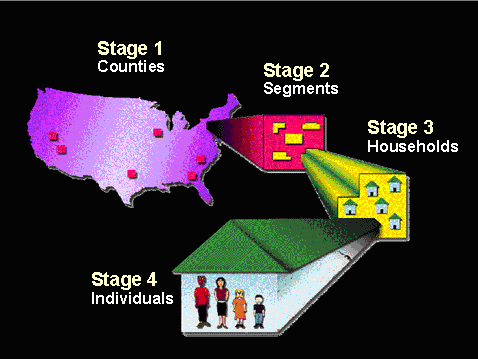
\includegraphics[width=0.75\textwidth]{figures/Survey_Design.PNG}
\caption{Multistage survey design used by NHANES. Note that the survey structure was Counties-Segments-Households-Individuals, in order of increasing specificity.}
\label{fig:survey.design}
\end{figure}

\begin{figure}[hp]
    \centering
    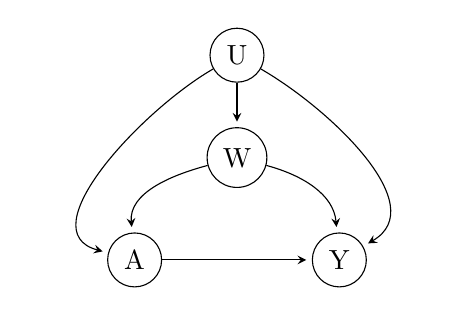
\begin{tikzpicture}[->, shorten >=2pt, >=stealth, node distance=1cm,
                        pil/.style={->,thick,shorten =2pt,},scale=0.65
                        ]
    \node[circle,draw] at (4,2) (1) {W};
    \node[circle,draw] at (2,0) (2) {A};
    \node[circle,draw] at (6,0) (3) {Y};
    \node[circle,draw] at (4,4) (4) {U};
    \draw[->] (1) to [out=195,in=95] (2);
    \draw[->] (2.east) -- (3.west);
    \draw[->] (1) to [out=345,in=95] (3);
    \draw[->] (4.south) -- (1.north);
    \draw[->] (4) to [out=210,in=165] (2);
    \draw[->] (4) to [out=330,in=30] (3);
    \end{tikzpicture}
  \caption{Simplified DAG -- no independence assumptions on $U$'s.}
  \label{fig:DAG}
\end{figure}


\begin{figure}
	\centering
    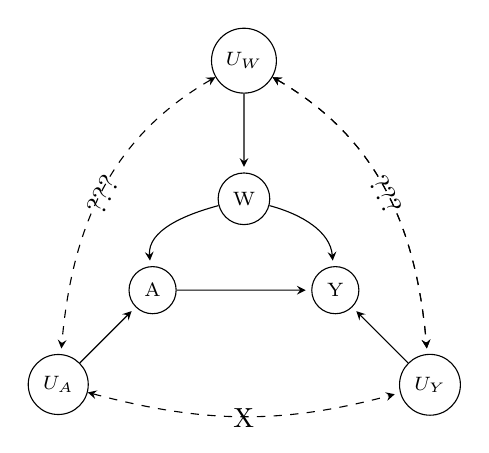
\begin{tikzpicture}[->, shorten >=2pt, >=stealth, node distance=1cm,
                        pil/.style={->,thick,shorten =2pt,},scale=0.65,font=\scriptsize
                        ]
    \node (A) [circle,draw] {A};
    \node (W) [circle,draw,above right=of A] {W};
    \node (Y) [circle,draw,below right=of W] {Y};
    \node (UA) [circle,draw,below left=of A] {$U_A$};
    \node (UW) [circle,draw,above=of W] {$U_W$};
    \node (UY) [circle,draw,below right=of Y] {$U_Y$};
    \draw[->] (W) to [out=195,in=95] (A);
    \draw[->] (A.east) -- (Y.west);
    \draw[->] (W) to [out=345,in=95] (Y);
    \draw[->] (UW.south) -- (W.north);
    \draw[->] (UA) to [out=45,in=225] (A);
    \draw[->] (UY) to [out=135,in=315] (Y);
    \draw[dashed,<->] (UW) to [out=330,in=95] (UY);
    %\pgftransformyshift{-.65cm}
    %\draw[decoration={text along path, text={X},text align={center}},decorate] (UA) to
                      [out=345,in=195] (UY);
    \draw[dashed,<->,postaction={decorate,decoration={raise=-4pt,text along path,text align=center,text={X}}}] (UA) to [out=345,in=195] (UY);
    \draw[dashed,<->,postaction={decorate,decoration={raise=-4pt,reverse path,text along path,text align=center,text={???}}}] (UW) to [out=210,in=85] (UA);
    \draw[dashed,<->,
    postaction={decorate,
    decoration={raise=-4pt,text along path,text align=center,text={???}}}] (UW) to [out=330,in=95] (UY);
    \end{tikzpicture}
\caption{DAG showing the backdoor criterion}
\label{fig:DAG1}
\end{figure}


\begin{figure}[hbp]
\centering
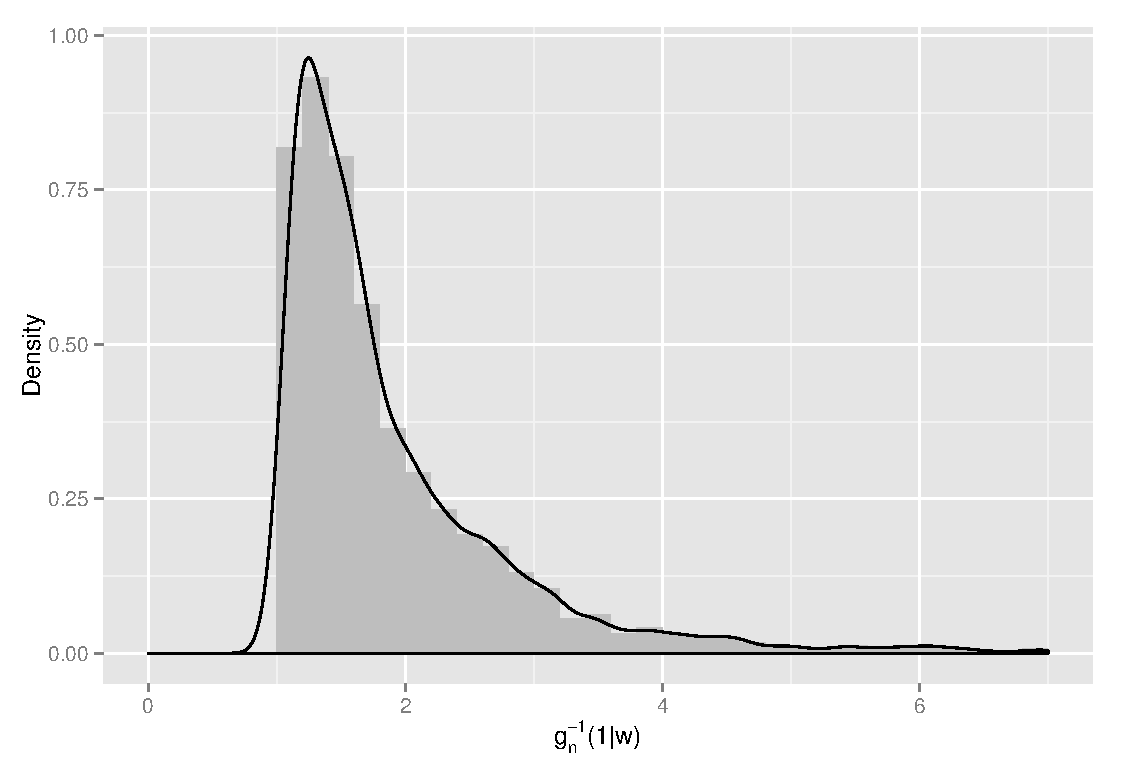
\includegraphics[width=0.75\textwidth]{figures/IPTWDensityPlot.pdf}
\caption{Histogram and Density estimate of weights from SuperLearner output. Here we truncate the x-axis at 7, but a summary of the full weight distribution can be seen in Table \ref{tab:weight.summary}, and a table of excluded values can be seen in Table \ref{tab:missing.weights}.}
\label{fig:weight.dist}
\end{figure}

\begin{table}
\centering
\begin{tabular}{c|c}
$x$ & number of individuals with weight $>x$ \\
\hline
8 & 13 \\
9 & 11 \\
10 & 10 \\
11 & 7 \\
13 & 5 \\
15 & 4 \\
16 & 2 \\
17 & 1
\end{tabular}
\caption{Table of Excluded values from density plot in Figure \ref{fig:weight.dist}}
\label{tab:missing.weights}
\end{table}

\begin{figure}
\centering
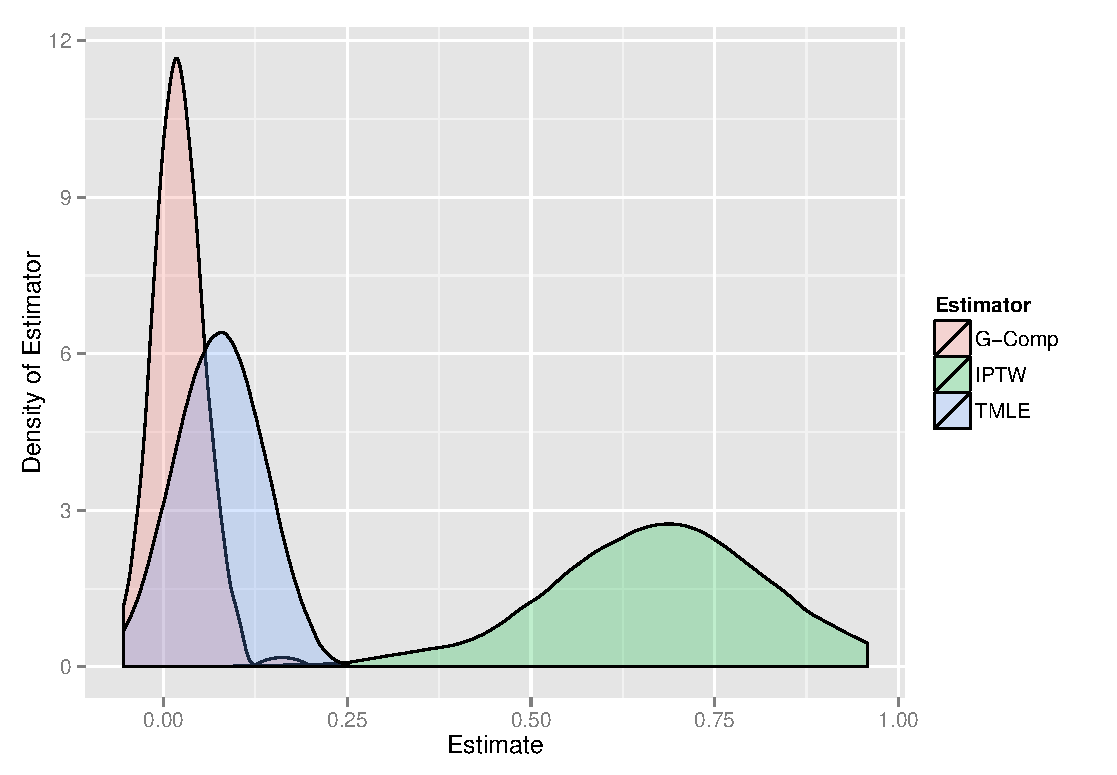
\includegraphics[width=0.75\textwidth]{figures/naiveBootstrapDensities.pdf}
\caption{Density estimates of the bootstrap distributions. Note that all of the distributions look approximately normal.}
\label{fig:boot.distr}
\end{figure}

\begin{figure}[hbp]
\centering
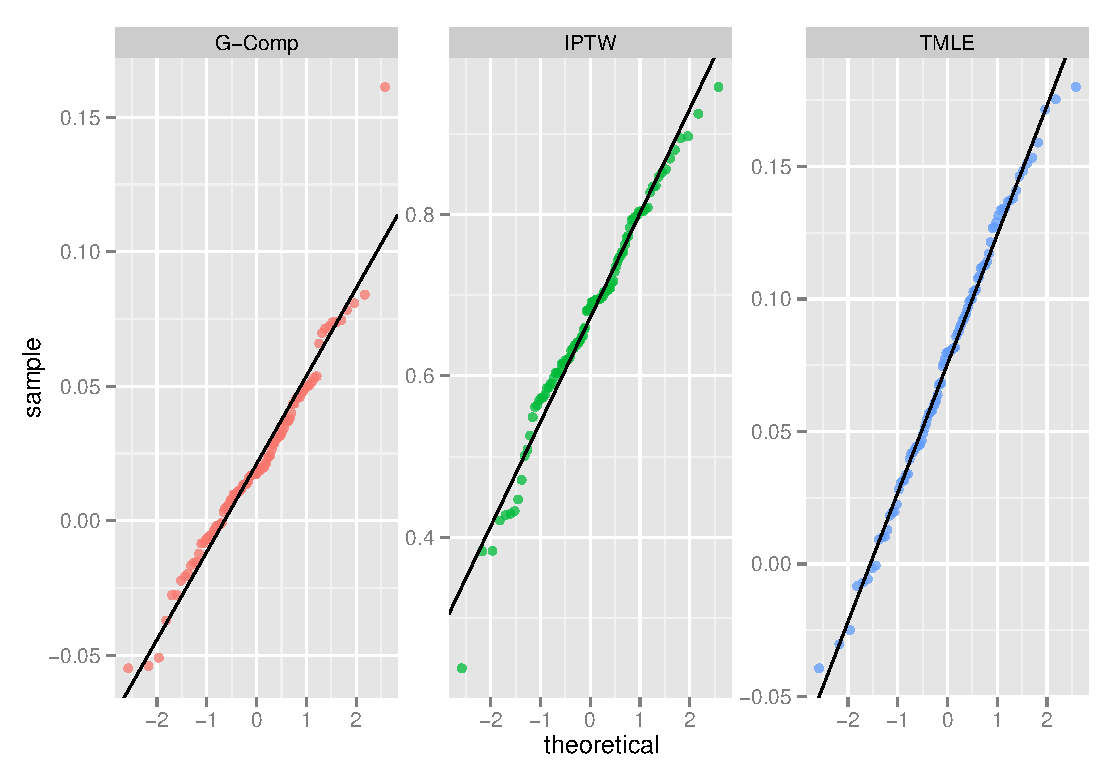
\includegraphics[width=0.9\textwidth]{figures/naiveBootstrapQQplots.pdf}
\caption{Q-Q plots for the bootstrap sampling distributions of the three estimators. Note that all of the estimators appear to fall along a straight line, indicating approximately normal data.}
\label{fig:qqplot}
\end{figure}


\begin{figure}
\centering
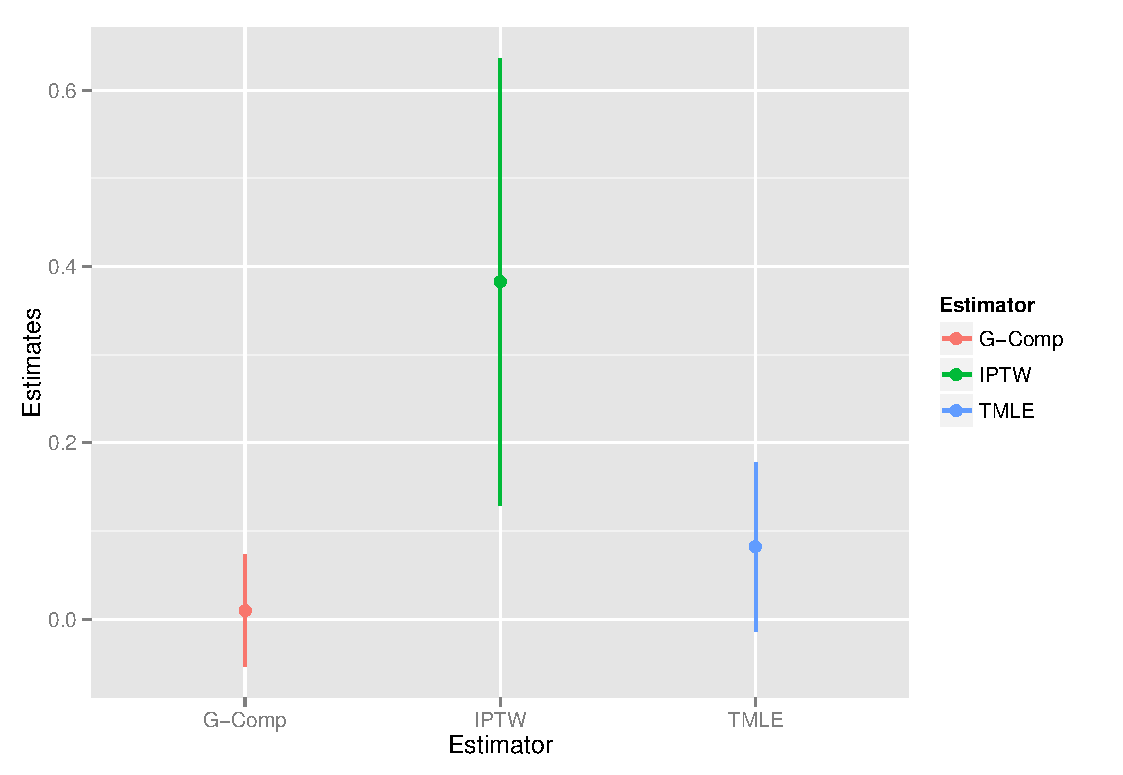
\includegraphics[width=0.75\textwidth]{figures/naiveBootstrapNormalCI.pdf}
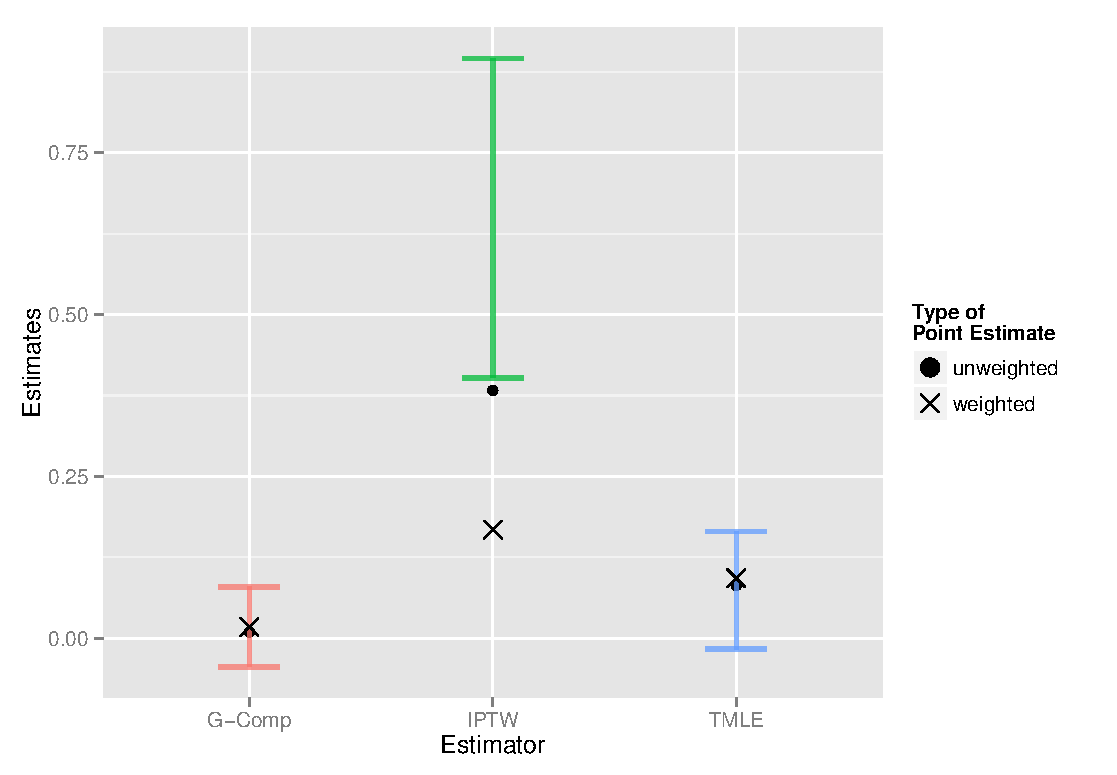
\includegraphics[width=0.75\textwidth]{figures/naiveBootstrapQuantileCI.pdf}
\caption{Plots of the 95\% confidence intervals for the estimates that do not incorporate survey weights. The confidence intervals derived from a normal approximation are on top, and those from the sample quantiles are below. Point estimates derived using survey weights are displayed for comparison purposes.}
\label{fig:cis}
\end{figure}

\end{document}
